\section{Executed Proseg diagnostics and width sensitivity}
Proseg 3.2.0 was run on both existing lung crops. The default factorization failed on the first crop with an empty-input feature-selection error; this failure also occurred with an equivalent CSV input. Both completed runs disabled factorization, while retaining upstream sampling defaults: 200 burn-in iterations, 200 sampling iterations and 50 hill-climb steps, with two CPU threads. This adaptation was motivated by execution failure before comparing assignment results.

The first crop retained 5,774 of 5,847 supplied transcripts and returned 93 cells; the second retained 1,482 of 1,523 and returned 72 cells. Source-owner disagreements on retained IDs numbered 3,242 and 765, respectively. Proseg assigned 2,484 and 1,335 retained molecules to background. These large background fractions underline the limitations of sparse, clipped inputs. Single-run executable times were 14.14 and 10.67 seconds, excluding installation and adapters. Neither agreement nor disagreement establishes accuracy, and these timings give no whole-slide performance claim.

The raw output, exact commands, input/output hashes and excluded transcript identifiers are preserved. Proseg cell indices are mapped through original cell IDs. Reach questions use shared retained molecule IDs, original observed coordinates and identical source/alternative count populations. Molecules omitted from a scored population remain geometric constraints with zero score. The nuclear reference retains its own border guard. Comparison denominators therefore remain reference-specific.

\subsection{Declared width sensitivity protocol}
The post-review protocol was recorded before the width runs, after the earlier atlas analyses. It uses the same two lung crops from one donor and makes no claim of preregistration before the original results. The three proposed chart halfwidth caps are $B=4,12,28$, with fallback ladders $(4,2,1,1/2)$, $(12,4,2,1,1/2)$ and $(28,4,2,1,1/2)$. The candidate ordering, label containment checks, disjointness checks, source masks and nuclear constraints remain fixed. Each atlas is re-extracted and independently checked with exact rational geometry. Both greedy selection and the different ladders mean that these families are non-nested. In particular, the largest ladder omits the intermediate halfwidth 12.

The source transform gives $p=1048576/4934475\,\mu\mathrm m$ per pixel. The chart-to-physical displacement is $p|h|/\sqrt2$ and the band is $|h|\le3B/4$. Each accepted atlas contains a patch with the proposed halfwidth cap. The corresponding displacement caps are upper bounds before additional slope and nuclear restrictions, rather than optimized attainable or typical displacements: halfwidth 12 is accepted in 132 of 544 intermediate-cap patches and halfwidth 28 in 41 of 543 largest-cap patches; all other accepted halfwidths are at most 4. No physical scale is inferred from a nominal image resolution. Counts, patch acceptance and coverage are reported below.

\begin{table}[ht]\centering
\begin{tabular}{lrrr}\toprule
Chart halfwidth cap $B$&4&12&28\\\midrule
Largest band displacement cap ($\mu\mathrm m$)&0.451&1.352&3.155\\
Accepted patches / candidates&544/782&544/782&543/782\\
Editable incident boundary edges (\%)&68.300&67.907&68.058\\
Editable transcripts&745&1,288&1,220\\
Nuclear changed counts reachable&186/1,134&223/1,134&190/1,134\\
Proseg changed counts reachable&185/2,798&241/2,798&200/2,798\\\bottomrule
\end{tabular}
\caption{Reach at unlimited area on fixed shared-observation populations. Each count is tested separately by exact score-spectrum membership; full alternative count matrices need not be jointly attainable. The largest cap loses some reach because the re-extracted families are non-nested.}
\end{table}

The declared area budgets, in $\mu\mathrm m^2$, are $0$, $0.01$, $0.025$, $0.05$, $0.075$, $0.1$, $0.15$, $0.2$, $0.25$, $0.3$, $0.4$, $0.5$, $0.75$, $1$, $2$ and $4$. The exact count minima allow both evaluation on this grid and unlimited-area membership. At cap 4, nuclear reach attains its unlimited value by budget 0.25 and Proseg reach by 0.2. At cap 12, both reach their unlimited values by budget 2. At cap 28, budget 4 reaches 189 nuclear and 197 Proseg counts, compared with unlimited values of 190 and 200. No timed-out or failed solve is reported as a certificate. All study runs completed, and independent checks found zero failures among 8,270 local count/geometry witnesses and 25,610 global count/area traces.

\begin{figure}[ht]\centering
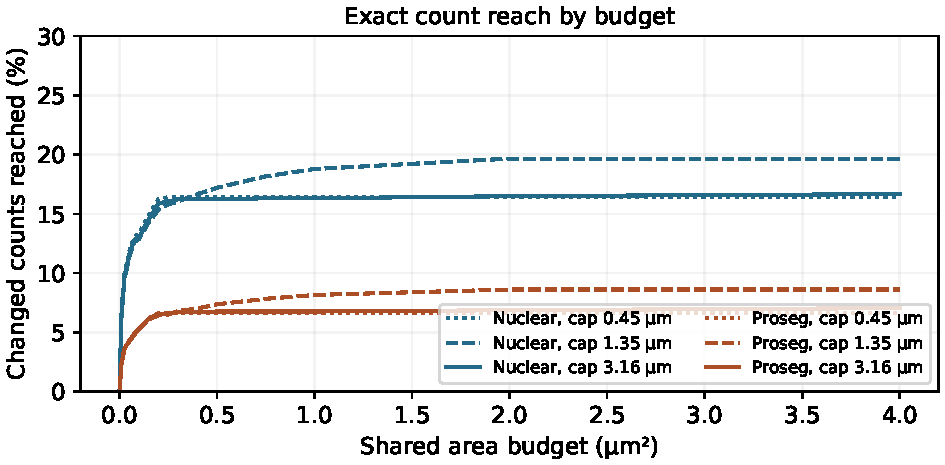
\includegraphics[width=.96\textwidth]{figures/reach_budget.pdf}
\caption{Exact reach as the shared area budget increases within each fixed width setting. Source and alternative counts use the same reference-specific retained molecule IDs. Curves from different width settings compare non-nested atlas families.}
\end{figure}

\subsection{Nuclear denominator audit}
The original nuclear comparison removed a gene whenever the five-micrometre crop-border guard intersected its editable spectrum. The width study scores only retained molecules, while keeping excluded molecules as zero-score geometric collateral. This permits six additional changed lung cell--gene questions in the default atlas. One, C7 in cell 153965, is reachable. Thus the refined default comparison is 186 of 1,134, compared with the original 185 of 1,128. Counts and reach agree for every previously shared question. The difference is an analysis-contract refinement, rather than an effect of increasing ribbon width. The audit preserves all six keys and their old/new inclusion status. The breast comparison retains the original protocol; it was not rerun across width settings.

The width study tests restricted geometric reach, rather than anatomical calibration. Each alternative count is assessed individually; reachable counts can still demand incompatible global assignments. Sparse clipped inputs, a single Proseg run per crop, adapted factorization and one lung donor limit interpretation. Source coordinates are held fixed, all transcript-ID exclusions are explicit, and agreement with an alternative segmenter supplies no ownership accuracy estimate.
